% vim: set spell spl=en:

\documentclass[portrait,final,a0paper,fontscale=0.27]{baposter}

\usepackage[utf8]{inputenc}
\usepackage[T1]{fontenc}

\usepackage{url}
\usepackage{caption}
\usepackage{tabularx}
\usepackage{graphicx}
\usepackage{multicol}
\usepackage{lipsum}
\usepackage{enumitem}
%\usepackage[vlined]{algorithm2e}
%\usepackage{algpseudocode}
\usepackage{algorithmic,etoolbox}


%\usepackage{times}
\usepackage{helvet}
%\usepackage{bookman}
%\usepackage{palatino}


% Multicol Settings
\setlength{\columnsep}{1.5em}
\setlength{\columnseprule}{0mm}

% Save space in lists. Use this after the opening of the list
\newcommand{\compresslist}{%
\setlength{\itemsep}{0pt}%
\setlength{\parskip}{0pt}%
\setlength{\parsep}{0pt}%
}

%%%%%%%%%%%%%%%%%%%%%%%%%%%%%%%%
% Begin of Document
%%%%%%%%%%%%%%%%%%%%%%%%%%%%%%%%

\renewcommand{\familydefault}{\sfdefault}

\begin{document}

%%%%%%%%%%%%%%%%%%%%%%%%%%%%%%%%%%%%%%%%%%%%%%%%%%%%%%%%%%%%%%%%%%%%%%%%%%%%%%
%%% Here starts the poster
%%%---------------------------------------------------------------------------
%%% Format it to your taste with the options
%%%%%%%%%%%%%%%%%%%%%%%%%%%%%%%%%%%%%%%%%%%%%%%%%%%%%%%%%%%%%%%%%%%%%%%%%%%%%%
% Define some colors

\definecolor{wlblue}{RGB}{62,153,210}
%\definecolor{alert}{RGB}{199,102,45}
\definecolor{alert}{RGB}{48,168,87}

\hyphenation{}

\def\alert#1{\textbf{\color{alert}#1}}

\background{%
    \begin{tikzpicture}
        [remember picture,overlay]\node[opacity=1.00] at (.295\paperwidth,.65\paperheight) {
\includegraphics[width=.67\paperwidth,height=0.67\paperheight]{wl-bg}};
    \end{tikzpicture}%
}


\begin{poster}  % Poster Options
  {
  % Show grid to help with alignment
  grid=false,
  columns=6,
  % Column spacing
  colspacing=1em,
  % Color style
  bgColorOne=white,
  bgColorTwo=white,
  borderColor=wlblue,
  headerColorOne=wlblue,
  headerColorTwo=wlblue,
  headerFontColor=white,
  boxColorOne=white,
  boxColorTwo=wlblue,
  % Format of textbox
  textborder=rectangle,
  % Format of text header
  eyecatcher=false,
  headerborder=closed,
  headerheight=0.1\textheight,
%  textfont=\sc, An example of changing the text font
  headershape=rectangle,
  headershade=shadelr,
  headerfont=\Large\bf\textsc, %Sans Serif
  textfont={\setlength{\parindent}{0em}},
  boxshade=plain,
%  background=shade-tb,
  background=user,
  linewidth=2pt,
  boxopacity=.5
  }
  % Eye Catcher
  {
    } 
  % Title
  {\bf\huge Virtualized Web Portals in EGI Federated Cloud}
  % Authors
  {\vspace{1em}\bf{Aleš Křenek, Radim Peša, Vlastimil Holer, Daniel Kouřil}

%	\medskip
%   {\normalfont\normalsize Institute of Computer Science, Masaryk University, Brno, Czech Republic
%
%	\bigskip
%}
}
  % University logo
  {% The makebox allows the title to flow into the logo, this is a hack because of the L shaped logo.
  
\includegraphics[height=4em]{wl-logo}
  }
  

%%%%%%%%%%%%%%%%%%%%%%%%%%%%%%%%%%%%%%%%%%%%%%%%%%%%%%%%%%%%%%%%%%%%%%%%%%%%%%
%%% Now define the boxes that make up the poster
%%%---------------------------------------------------------------------------
%%% Each box has a name and can be placed absolutely or relatively.
%%% The only inconvenience is that you can only specify a relative position 
%%% towards an already declared box. So if you have a box attached to the 
%%% bottom, one to the top and a third one which should be in between, you 
%%% have to specify the top and bottom boxes before you specify the middle 
%%% box.
%%%%%%%%%%%%%%%%%%%%%%%%%%%%%%%%%%%%%%%%%%%%%%%%%%%%%%%%%%%%%%%%%%%%%%%%%%%%%%
    %
    % A coloured circle useful as a bullet with an adjustably strong filling
    \newcommand{\colouredcircle}{%
      \tikz{\useasboundingbox (-0.2em,-0.32em) rectangle(0.2em,0.32em); \draw[draw=black,fill=lightgreen,line width=0.03em] (0,0) circle(0.18em);}}

\headerbox{}{name=logos,column=0,span=6,above=bottom,textborder=none,headerborder=none,boxheaderheight=0pt}
{
\noindent

\includegraphics[height=3em]{eu}

\includegraphics[height=3em]{h2020}

\includegraphics[height=3em]{einfra}
\hfill
\vbox{
\raggedleft
\hsize=.4\hsize
Contact: \url{ljocha@ics.muni.cz}
\smallskip

Further information at \url{http://bit.ly/2mBDjD1}
\par
}
\ 
\includegraphics[height=3em]{qr}
}


%%%%%%%%%%%%%%%%%%%%%%%%%%%%%%%%%%%%%%

% 
%%%%%%%%%%%%%%%%%%%%%%%%%%%%%%%%%%



%%%%%%%%%%%%%%%%%%%%%%%%%%%%%%%%%%%%%%%%%%%%%%%%%%%%%%%%%%%%%%%%%%%%%%%%%%%%%%
\headerbox{Go to Cloud}{name=virt,column=3,row=0,span=3}
{

\parskip=\medskipamount
Cloud infrastructures available nowadays, together with cloud orchestration
engines allow \alert{addressing those issues} in a scalable way. 

Rather than
maintaining ``one size fits all'' instance of an application web portal, we
provide \alert{templates for deployment} multiple instances of a specific portal,
dedicated to smaller user groups. 

Instances may vary in size, and they can
be easily customized to the needs of their users, while still reusing 99\% of
the common code and configuration.

Deployment is \alert{easily reproducible}, making maintenance easier.

User groups are \alert{isolated from one another} more thoroughly.

}

\headerbox{Web Portals Pros and Cons}{name=portal,column=0,row=0,span=3,bottomaligned=virt}{

\parskip=\medskipamount
Applicaton web portals, popular in many areas, \alert{shield the user from complexity}
of application workflow implementation and control of computing resources.

On the other hand, implementation of such web portal itself involves \alert{rather
complicated} technology, which becomes \alert{difficult to operate and maintain} as the
number of its users grows. 

Moreover, users may come with
\alert{mutually contradictory requirements}
(e.g. stick with an old version of simulation software to retain full backward
compatibility vs.\ use a new version to leverage new features).

}

%%%%%%%%%%%%%%%%%%%%%%%%%%%%%%%%%
\headerbox{Architecture and Typical Deplyoment}{name=arch,column=0,below=portal,span=6}
{
\begin{multicols}4
\textbf{Group admin view}
\begin{enumerate}
\item User group negotiates access to cloud site
\item Resource templates are created to match 
available resources and application software
\item AuthN metadata are exchanged with Westlife IdP-SP proxy
\item Group IT manager spawns orchestrated deployment
\item Virtual machines are created automatically
\item Minimalistic OS images are used, software is installed on instantiation
\end{enumerate}

\vfill
\columnbreak
\ 
\vfill
\begin{minipage}[c][20em]{2\columnwidth+1\columnsep}
\centering
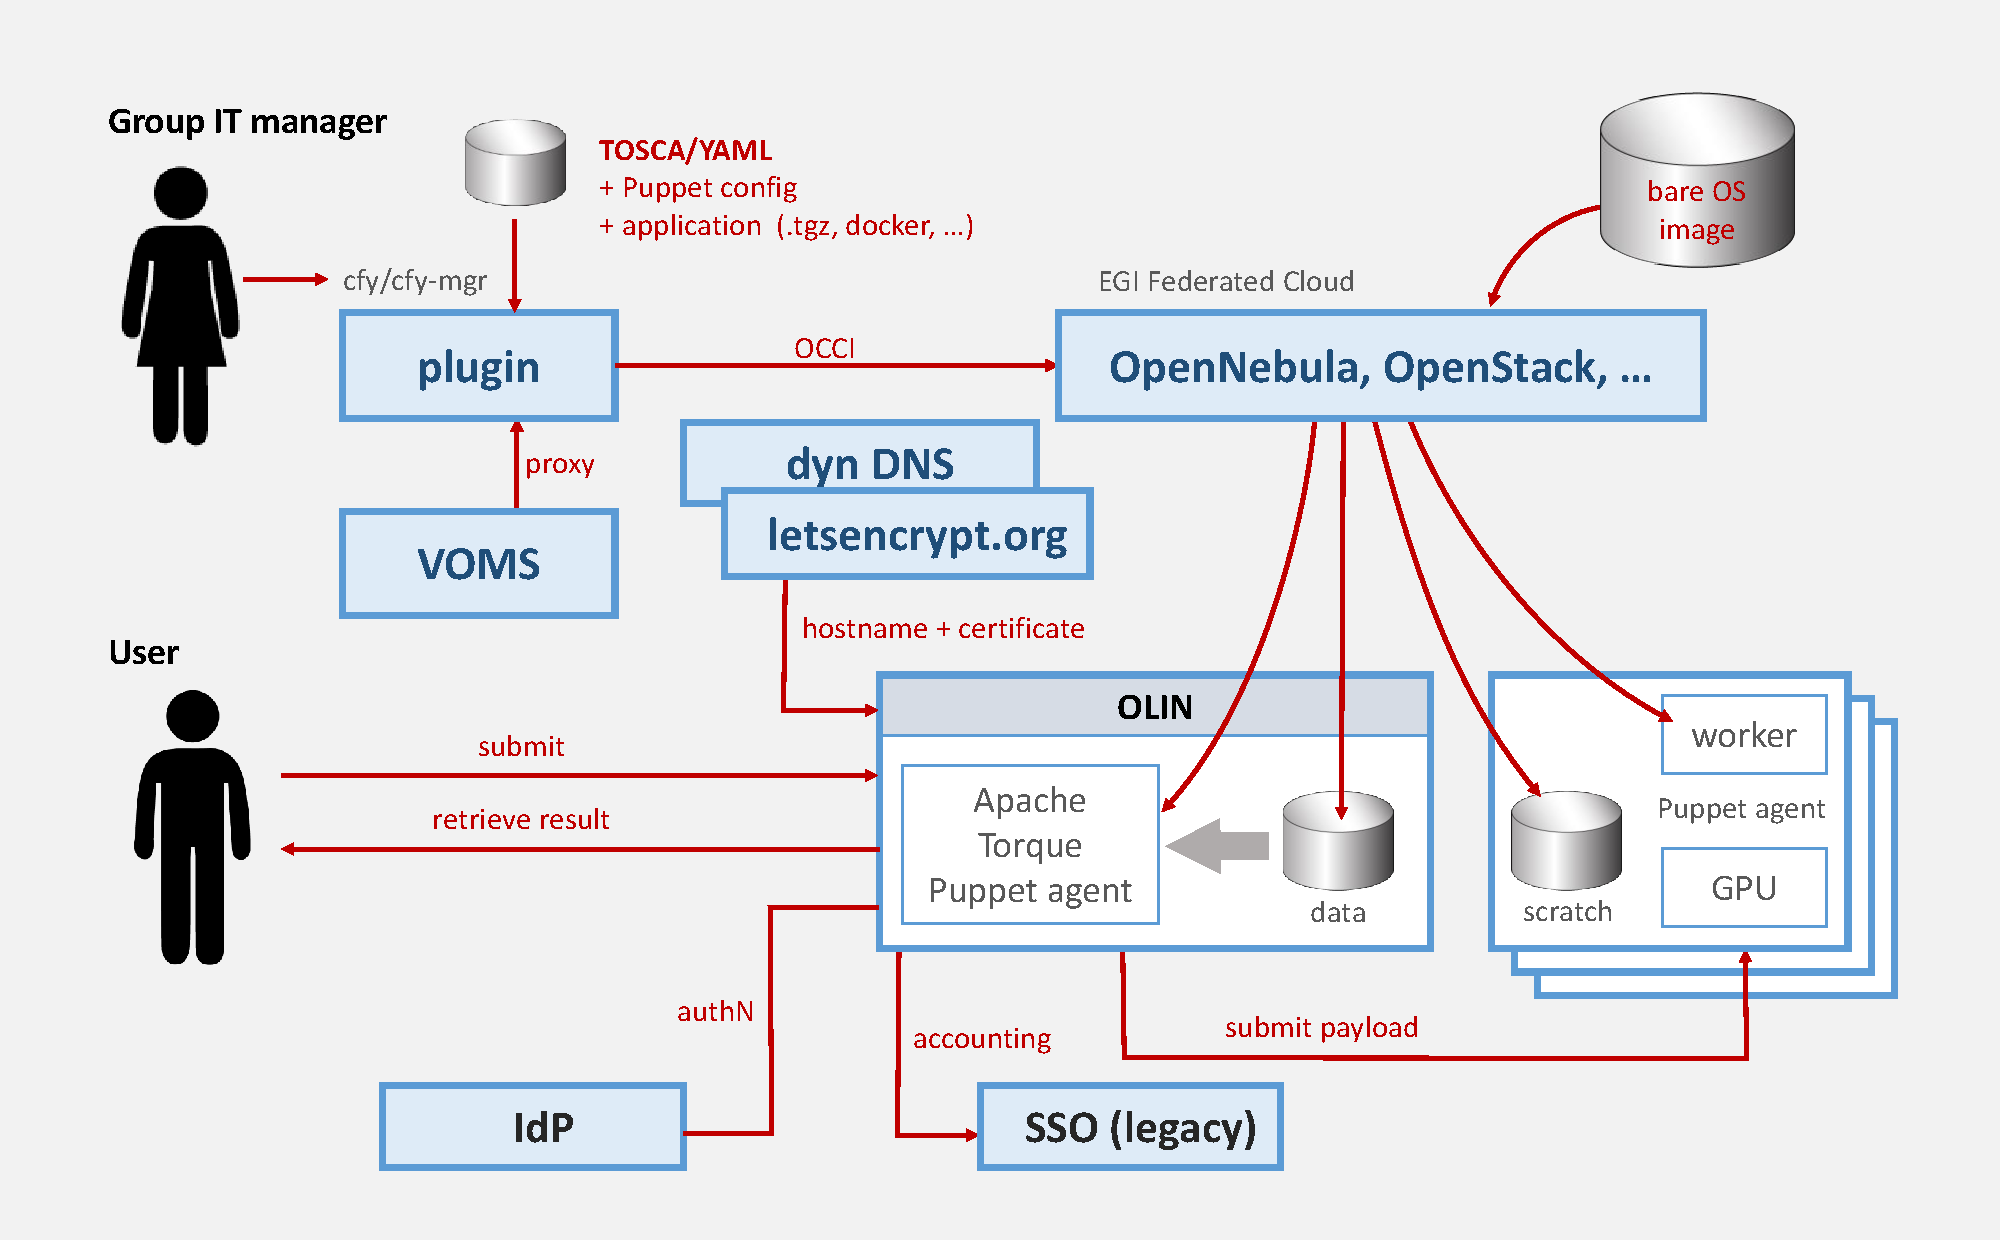
\includegraphics[width=\hsize]{schema_export}
\end{minipage}

\vfill
\columnbreak

\ 

\columnbreak

\raggedright
\textbf{User view}
\begin{enumerate}
\item Users authenticate with ``home'' identities or Google/Facebook
\item Jobs are accepted by web interface front-end
\item Portal may have specific features requested by this group
\item Computation is run on virtual cluster, hidden to the user
\item Virtual cluster size can be adapted to the load dynamically

\end{enumerate}
\vfill
\ 
\end{multicols}
}

\headerbox{Usecases}%
{name=acknow, column=4, span=2, below=arch,above=logos}%
{ 
New version of \alert{Gromacs} molecular dynamics portal, based on \alert{version 5.1},
with support of GPU, is the pilot application.

\medskip
We work on adaptation of \alert{Scipion} CryoEM data processing, its Web Tools variant first, with foreseen support of the full version.

\medskip
Cloudified approach will be leveraged to address \alert{workflow usecases} of Westlife project,
integration of Scipion and Powerfit specifically.

\medskip
With \alert{FireProt} protein thermal stability workflow the cloudified version brings another benefit
-- the sofware can be used by \alert{pharma companies} in a~strictly controlled environment.

\medskip
In \alert{EDIReX project}, several replicated instances will be used to control
access to \alert{sensitive data}.

}

\headerbox{Common Technology}{name=tech,column=0,below=arch,span=4}
{
\begin{itemize}

\item Portal virtual cluster is described by \alert{TOSCA} specification.

\item Deployment is controlled by \alert{Cloudify} orchestration tools.
% \url{http://getcloudify.org}

\item Access to the cloud site is authenticated with \alert{X.509 certificate} and \alert{VOMS proxy}, 
virtual machines are controlled by \alert{OCCI} Cloudify plugin.

\item Software configuration at cluster nodes is managed by \alert{Puppet}.

\item Typically, \alert{Apache} web server and \alert{Torque} batch systems are used.

\item \alert{GPU} can be leveraged if available and supported by the application.

\item Users authenticate with identity federation through \alert{Shibboleth}.

\item Future migration to \alert{INDIGO Datacloud} orchestration tools is foreseen.

\end{itemize}
}

\headerbox{Acknowledgement}{name=use,column=0,below=tech,above=logos,span=4}
{
This work was done in the West-life project, part of 
e-Infrastructures for virtual research environments (VRE), project Number 675858

Computing resources were provided by CERIT Scientific Cloud
centre within project no. LM2015085.
}

\end{poster}
\end{document}
